%\documentclass[svgnames]{beamer}
\documentclass[svgnames, handout,t]{beamer}

\usefonttheme[onlymath]{serif}		% Display math in serif font

%\usepackage[svgnames]{xcolor}

\batchmode
% \usepackage{pgfpages}
% \pgfpagesuselayout{4 on 1}[letterpaper,landscape,border shrink=5mm]

\usepackage{amsmath,amssymb,color}

\usetheme{Berlin}
\usecolortheme{bear}

\title{Compact implementations of pairings}
\author[Anthony Van Herrewege]{Anthony Van Herrewege\\[2em]
\small Lejla Batina \& Miroslav Knezevic\\
Prof. Dr. Ir. I. 	Verbauwhede \& Prof. Dr. Ir. B. Preneel}
\date{22 May 2009}
%\pgfdeclareimage[height=1cm]{brown-logo}{brown-logo.pdf}
%\logo{\pgfuseimage{brown-logo}\hspace*{0.3cm}}

\AtBeginSection[]
{
  \begin{frame}<beamer>
    \frametitle{Outline}
    \tableofcontents[currentsection]
  \end{frame}
}
\beamerdefaultoverlayspecification{<+->}

\begin{document}

\frame{\titlepage}

\section[Outline]{}
\begin{frame}{Outline}
  \tableofcontents
\end{frame}

\section{Problem}
\subsection*{Problem}
\begin{frame}{Symmetric cryptography}
	\begin{itemize}
		\item Pro:
			\begin{itemize}
				\item High security per bit
				\item Very fast implementations
			\end{itemize}
		\item Contra:
			\begin{itemize}
				\item How to establish the key?
			\end{itemize}		
	\end{itemize}
\end{frame}

\begin{frame}{Asymmetric cryptography}
	\begin{itemize}
		\item Pro:
			\begin{itemize}
				\item No key establishment necessary
				\item Central location with everyone's key
			\end{itemize}
		\item Contra:
			\begin{itemize}
				\item Need for certificate authorities, \ldots
			\end{itemize}		
	\end{itemize}
\end{frame}

\begin{frame}{Identity-based cryptography}
	\begin{itemize}
		\item Pro:
			\begin{itemize}
				\item Public key deduced from ID
				\item No need for certificates
			\end{itemize}
		\item Contra:
			\begin{itemize}
				\item How to issue new keys, \ldots ?
			\end{itemize}
		\item Extra's:
			\begin{itemize}
				\item Non-interactive key establishment
				\item Date-stamped encryption
			\end{itemize}
	\end{itemize}
\end{frame}

\section{Pairings}
\subsection*{Pairings}
\begin{frame}{What?}
	\begin{itemize}
		\item Mathematical construction discovered in the 40's
		\item Allow implementation of ID-based cryptography
		\item Strength based on discrete logarithm problem
	\end{itemize}
\end{frame}

\begin{frame}{How?}
	Several available pairings:
	\begin{center}Weil, \alert{Tate}, ate, eta, $\ldots$\end{center}
	
	Tate pairing:	
	\[ \hat{e}(P, Q) : E(\mathbb{F}_q)[l] \times E(\mathbb{F}_q)[l] \mapsto \mu _l \]
	
	Mapping needs to be:	
	\begin{itemize}
		\item<1-> Bilinear: $\hat{e}(P_1 + P_2, Q) = e(P_1, Q) \cdot e(P_2, Q)$
		\item<1-> Non-degenerate: $\hat{e}(P, P) \neq 1$
		\item<1-> Efficiently computable
	\end{itemize}
	

\end{frame}

\section{Implementation}
\subsection*{Implementation}
\begin{frame}{MALU}
	Modulo Arithmetic Logical Unit [general]:\\[8mm]
	\begin{center}
		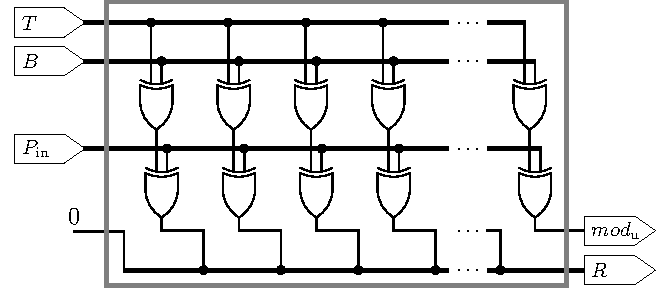
\includegraphics[height=0.5\paperheight]{images/malu-basic}
	\end{center}
\end{frame}

\begin{frame}{MALU}
	Modulo Arithmetic Logical Unit [optimized]:\\[3mm]
	\begin{center}
		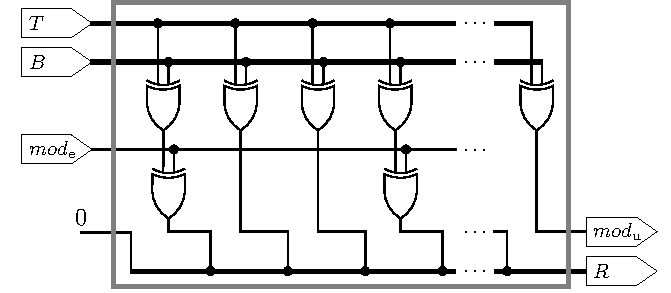
\includegraphics[height=0.5\paperheight]{images/malu-optimized}
	\end{center}
\end{frame}

\begin{frame}{MALU}
	Modulo Arithmetic Logical Unit [optimized; d-bits wide]:\\
	\begin{center}
		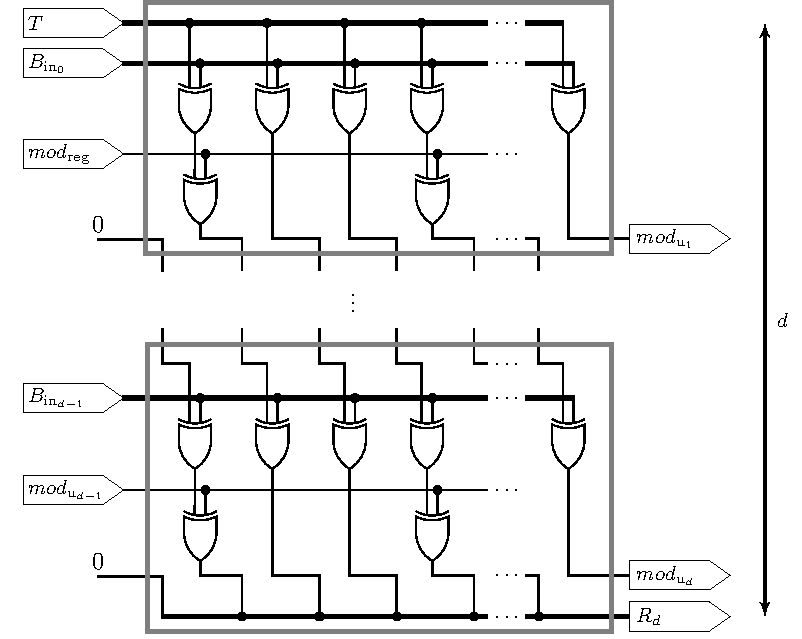
\includegraphics[height=0.55\paperheight]{images/malu-width-d}
	\end{center}
\end{frame}

\begin{frame}{Wrappers - $GF_{2^m}$}
	$GF_{2^m}$ Multiplication/Addition:\\
	\begin{center}
		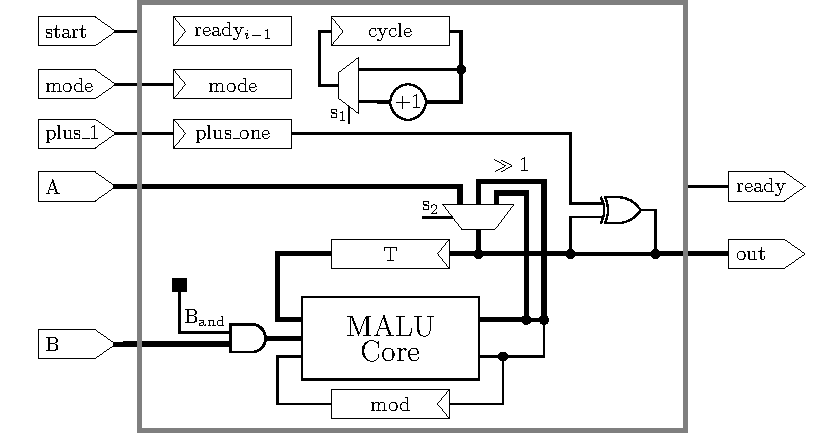
\includegraphics[height=0.55\paperheight]{images/wrapper-gf2m}
	\end{center}
\end{frame}

\begin{frame}{Controller - Miller's algorithm}
	\vfill
	\centering
		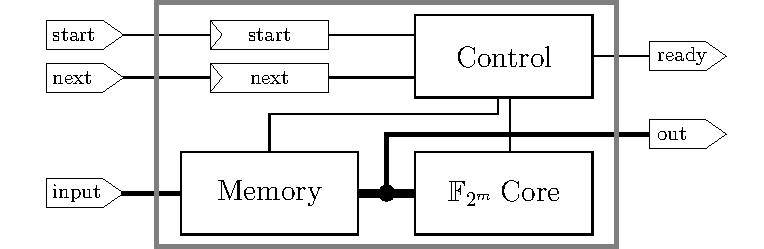
\includegraphics[width=0.8\paperwidth]{images/controller-miller}
	\vfill
\end{frame}

\begin{frame}{State of the art}
	Some currently available implementations:\\
	
	\begin{center}
	\begin{tabular}{llll}
		Name		&	Platform	&	Field	&	Speed\\
		\hline
		TinyTate		&	ATMega128L [7.4Mhz]	& $\mathbb{F}_{2^{256}}$	& 30.2s\\
		TinyPBC		&	ATMega128L [7.4Mhz]	& $\mathbb{F}_{2^{256}}$	& 5.45s\\
		Hankerson	&	P4 [2.8Ghz]				& $\mathbb{F}_{2^{1223}}$	& 0.07s\\
		Hankerson	&	P4 [2.8Ghz]	(SSE) 	& $\mathbb{F}_{2^{1223}}$	& 0.03s\\
		\end{tabular}
	\end{center}
\end{frame}

\section{Conclussion}
\subsection*{Conclussion}
\begin{frame}{Progress so far}
	\begin{itemize}
		\item<1-> MALU
		\item<1->	$GF_{2^m}$ functions
		\item<1-> ECC functions
		\item<1-> Pairing functions (partial)
	\end{itemize}
\end{frame}

\begin{frame}{To do}
	\begin{itemize}
		\item<1-> Complete pairing functions
		\item<1-> Bugfixing
		\item<1-> Optimization (VHDL)
		\item<1-> Write thesis text
	\end{itemize}
\end{frame}

\begin{frame}{The end}
	\begin{center}\LARGE Questions?\end{center}
\end{frame}

\end{document}
